% Previous horizontal figure preserved for review:
% % Native TikZ source for Figure~\ref{fig:bg-alternative-lookup-hits}.
% % Values: vcomp/experiments/results/
% %         paper_figure4_uniform_read_cache_5m_single.tsv
% % Configuration: D_pinned_5pct; successful lookups are
% % rocksdb.bloom.filter.full.true.positive / completed operations.
% \definecolor{altHitBaseline}{HTML}{5B5B5B}
% \definecolor{altHitFlush}{HTML}{E69F00}
% \definecolor{altHitLast}{HTML}{F0A83B}
% \definecolor{altHitFill}{HTML}{009E73}
% \definecolor{altHitFillOW}{HTML}{4AAE91}
% \definecolor{altHitFTwo}{HTML}{0072B2}
% 
% \begin{tikzpicture}[
%     x=1cm,
%     y=1cm,
%     font=\rmfamily,
%     bar/.style={draw=black, line width=0.45pt}
% ]
% \path[use as bounding box] (-0.05,-0.70) rectangle (3.10,4.70);
% 
% % Plot region: x=0.35 is 0%, x=2.60 is 100%.
% \foreach \x in {0.35,1.475,2.60} {
%     \draw[black!18, line width=0.45pt] (\x,0.30) -- (\x,4.42);
% }
% \draw[black, line width=0.60pt] (0.35,0.30) -- (2.72,0.30);
% \draw[black, line width=0.60pt] (0.35,0.30) -- (0.35,4.42);
% 
% % Baseline=63.214%, Flush-only=63.314%, Last-comp=63.214%,
% % Fillseq=100%, Fillseq+OW=100%, F2Load=61.761%.
% \draw[bar, fill=altHitBaseline] (0.35,3.88) rectangle (1.772,4.28);
% \node[font=\scriptsize, anchor=west] at (1.82,4.08) {63\%};
% 
% \draw[bar, fill=altHitFlush] (0.35,3.18) rectangle (1.775,3.58);
% \node[font=\scriptsize, anchor=west] at (1.82,3.38) {63\%};
% 
% \draw[bar, fill=altHitLast] (0.35,2.48) rectangle (1.772,2.88);
% \node[font=\scriptsize, anchor=west] at (1.82,2.68) {63\%};
% 
% \draw[bar, fill=altHitFill] (0.35,1.78) rectangle (2.60,2.18);
% \node[font=\scriptsize, anchor=east] at (2.56,1.98) {100\%};
% 
% \draw[bar, fill=altHitFillOW] (0.35,1.08) rectangle (2.60,1.48);
% \node[font=\scriptsize, anchor=east] at (2.56,1.28) {100\%};
% 
% \draw[bar, fill=altHitFTwo] (0.35,0.38) rectangle (1.740,0.78);
% \node[font=\scriptsize, anchor=west] at (1.79,0.58) {62\%};
% 
% \foreach \y in {0.58,1.28,1.98,2.68,3.38,4.08} {
%     \draw[black, line width=0.55pt] (0.27,\y) -- (0.35,\y);
% }
% \node[font=\scriptsize, anchor=north] at (0.35,0.18) {0};
% \node[font=\scriptsize, anchor=north] at (1.475,0.18) {50};
% \node[font=\scriptsize, anchor=north] at (2.60,0.18) {100};
% \node[font=\small, anchor=north] at (1.48,-0.28)
%     {Successful lookups (\%)};
% \end{tikzpicture}

% Previous plotted version preserved for review:
% % Loading: vcomp/experiments/results/paper_figure4_loading_time_1tb_single.tsv
% % Reads: vcomp/experiments/results/paper_figure4_uniform_read_cache_5m_single.tsv
% % One run per cell; all measured values are unchanged by this layout revision.
% \begingroup
% \definecolor{vb0}{HTML}{5B5B5B}
% \definecolor{vb1}{HTML}{E69F00}
% \definecolor{vb2}{HTML}{F0A83B}
% \definecolor{vb3}{HTML}{009E73}
% \definecolor{vb4}{HTML}{4AAE91}
% \definecolor{vb5}{HTML}{0072B2}
% \begin{tikzpicture}[x=1cm,y=1cm,font=\small,
% axis/.style={draw=black!80,line width=0.5pt},
% grid/.style={draw=black!16,line width=0.4pt}]
% \path[use as bounding box] (0,0) rectangle (5.200,5.650);
% \draw[grid] (0.85,1.4000) -- (5.1300,1.4000);
% \draw[axis] (0.79,1.4000) -- (0.85,1.4000);
% \node[font=\fontsize{7}{8}\selectfont,anchor=east] at (0.7300,1.4000) {0};
% \draw[grid] (0.85,2.8348) -- (5.1300,2.8348);
% \draw[axis] (0.79,2.8348) -- (0.85,2.8348);
% \node[font=\fontsize{7}{8}\selectfont,anchor=east] at (0.7300,2.8348) {50};
% \draw[grid] (0.85,4.2696) -- (5.1300,4.2696);
% \draw[axis] (0.79,4.2696) -- (0.85,4.2696);
% \node[font=\fontsize{7}{8}\selectfont,anchor=east] at (0.7300,4.2696) {100};
% \draw[axis] (0.85,1.4000) -- (5.1300,1.4000);
% \draw[axis] (0.85,1.4000) -- (0.85,4.7000);
% \node[font=\fontsize{7}{8}\selectfont,rotate=90,anchor=south] at (0.1000,3.0500) {Successful lookups (\%)};
% % baseline: successful lookups=63.214418500%
% \draw[draw=black!80,line width=0.4pt,fill=vb0] (1.01000,1.40000) rectangle (1.45000,3.21398);
% \node[font=\fontsize{7}{8}\selectfont,anchor=south] at (1.2300,3.2840) {63.2};
% \node[font=\fontsize{7}{8}\selectfont,rotate=55,anchor=north east] at (1.2300,1.3000) {Baseline};
% % flush_only: successful lookups=63.314255400%
% \draw[draw=black!80,line width=0.4pt,fill=vb1] (1.71000,1.40000) rectangle (2.15000,3.21684);
% \node[font=\fontsize{7}{8}\selectfont,anchor=south] at (1.9300,3.2868) {63.3};
% \node[font=\fontsize{7}{8}\selectfont,rotate=55,anchor=north east] at (1.9300,1.3000) {Flush-only};
% % last_comp: successful lookups=63.214061100%
% \draw[draw=black!80,line width=0.4pt,fill=vb2] (2.41000,1.40000) rectangle (2.85000,3.21397);
% \node[font=\fontsize{7}{8}\selectfont,anchor=south] at (2.6300,3.2840) {63.2};
% \node[font=\fontsize{7}{8}\selectfont,rotate=55,anchor=north east] at (2.6300,1.3000) {Last-comp};
% % fillseq: successful lookups=100.000000000%
% \draw[draw=black!80,line width=0.4pt,fill=vb3] (3.11000,1.40000) rectangle (3.55000,4.26957);
% \node[font=\fontsize{7}{8}\selectfont,anchor=south] at (3.3300,4.3396) {100};
% \node[font=\fontsize{7}{8}\selectfont,rotate=55,anchor=north east] at (3.3300,1.3000) {Fillseq};
% % fillseq_ow: successful lookups=100.000000000%
% \draw[draw=black!80,line width=0.4pt,fill=vb4] (3.81000,1.40000) rectangle (4.25000,4.26957);
% \node[font=\fontsize{7}{8}\selectfont,anchor=south] at (4.0300,4.3396) {100};
% \node[font=\fontsize{7}{8}\selectfont,rotate=55,anchor=north east] at (4.0300,1.3000) {Fillseq+OW};
% % f2load: successful lookups=61.761495000%
% \draw[draw=black!80,line width=0.4pt,fill=vb5] (4.51000,1.40000) rectangle (4.95000,3.17229);
% \node[font=\fontsize{7}{8}\selectfont,anchor=south] at (4.7300,3.2423) {61.8};
% \node[font=\fontsize{7}{8}\selectfont,rotate=55,anchor=north east] at (4.7300,1.3000) {F2Load};
% \end{tikzpicture}
% \endgroup

% Active vertical figure generated from the promoted TSV data.
% Loading: vcomp/experiments/results/paper_figure4_loading_time_1tb_single.tsv
% Reads: vcomp/experiments/results/paper_figure4_uniform_read_cache_5m_single.tsv
% One run per cell; labels, membership and ratios derive from the TSV inputs.
\begingroup
\definecolor{vb0}{HTML}{5B5B5B}
\definecolor{vb1}{HTML}{E69F00}
\definecolor{vb2}{HTML}{F0A83B}
\definecolor{vb3}{HTML}{009E73}
\definecolor{vb4}{HTML}{4AAE91}
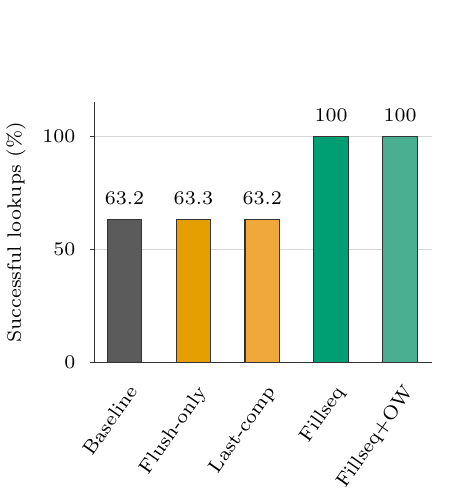
\begin{tikzpicture}[x=1cm,y=1cm,font=\small,
axis/.style={draw=black!80,line width=0.5pt},
grid/.style={draw=black!16,line width=0.4pt}]
\path[use as bounding box] (0,0) rectangle (5.200,5.650);
\draw[grid] (0.85,1.4000) -- (5.1300,1.4000);
\draw[axis] (0.79,1.4000) -- (0.85,1.4000);
\node[font=\fontsize{7}{8}\selectfont,anchor=east] at (0.7300,1.4000) {0};
\draw[grid] (0.85,2.8348) -- (5.1300,2.8348);
\draw[axis] (0.79,2.8348) -- (0.85,2.8348);
\node[font=\fontsize{7}{8}\selectfont,anchor=east] at (0.7300,2.8348) {50};
\draw[grid] (0.85,4.2696) -- (5.1300,4.2696);
\draw[axis] (0.79,4.2696) -- (0.85,4.2696);
\node[font=\fontsize{7}{8}\selectfont,anchor=east] at (0.7300,4.2696) {100};
\draw[axis] (0.85,1.4000) -- (5.1300,1.4000);
\draw[axis] (0.85,1.4000) -- (0.85,4.7000);
\node[font=\fontsize{7}{8}\selectfont,rotate=90,anchor=south] at (0.1000,3.0500) {Successful lookups (\%)};
% baseline: successful lookups=63.211859098%
\draw[draw=black!80,line width=0.4pt,fill=vb0] (1.01000,1.40000) rectangle (1.45000,3.21391);
\node[font=\fontsize{7}{8}\selectfont,anchor=south] at (1.2300,3.2839) {63.2};
\node[font=\fontsize{7}{8}\selectfont,rotate=55,anchor=north east] at (1.2300,1.3000) {Baseline};
% flush_only: successful lookups=63.270297782%
\draw[draw=black!80,line width=0.4pt,fill=vb1] (1.88500,1.40000) rectangle (2.32500,3.21558);
\node[font=\fontsize{7}{8}\selectfont,anchor=south] at (2.1050,3.2856) {63.3};
\node[font=\fontsize{7}{8}\selectfont,rotate=55,anchor=north east] at (2.1050,1.3000) {Flush-only};
% last_comp: successful lookups=63.213520422%
\draw[draw=black!80,line width=0.4pt,fill=vb2] (2.76000,1.40000) rectangle (3.20000,3.21395);
\node[font=\fontsize{7}{8}\selectfont,anchor=south] at (2.9800,3.2840) {63.2};
\node[font=\fontsize{7}{8}\selectfont,rotate=55,anchor=north east] at (2.9800,1.3000) {Last-comp};
% fillseq: successful lookups=100.000000000%
\draw[draw=black!80,line width=0.4pt,fill=vb3] (3.63500,1.40000) rectangle (4.07500,4.26957);
\node[font=\fontsize{7}{8}\selectfont,anchor=south] at (3.8550,4.3396) {100};
\node[font=\fontsize{7}{8}\selectfont,rotate=55,anchor=north east] at (3.8550,1.3000) {Fillseq};
% fillseq_ow: successful lookups=100.000000000%
\draw[draw=black!80,line width=0.4pt,fill=vb4] (4.51000,1.40000) rectangle (4.95000,4.26957);
\node[font=\fontsize{7}{8}\selectfont,anchor=south] at (4.7300,4.3396) {100};
\node[font=\fontsize{7}{8}\selectfont,rotate=55,anchor=north east] at (4.7300,1.3000) {Fillseq+OW};
\end{tikzpicture}
\endgroup
